\chapter{Regression}

% ---------- MAE ----------
\clearpage
\thispagestyle{regressionstyle}
\section{MAE}
\subsection{Mean Absolute Error}

MAE is one of the most popular regression accuracy metrics. It is calculated as the sum of absolute errors divided by the sample size. 
It is a scale-dependent accuracy measure which means that it uses the same scale as the data being measured.

% equation
\begin{center}
    \tikz{
        \node[inner sep=2pt, font=\Large] (a) {
            {
                $\displaystyle
                MAE = \frac{1}{{\color{nmlred}n}} \sum_{t=1}^n |{\color{nmlcyan}Y_t} - {\color{nmlpurple}\hat{Y}_t}|
                $
            }
        };
        \draw[-latex,nmlred, semithick] ($(a.south)+(-0.4,0.2)$) to[bend left=15] node[pos=1, left] {number of samples} +(-1,-.5);
        \draw[-latex,nmlpurple, semithick] ($(a.north)+(2.2,-0.3)$) to[bend left=15] node[pos=1, right] {forecast value} +(1,.5); 
        \draw[-latex,nmlcyan, semithick] ($(a.south)+(1.2,0.5)$) to[bend right=15] node[pos=1, right] {actual value} +(1,-.5);
    }
\end{center}

The smaller the MAE, the closer the model's predictions are to the actual targets.
Theoretically, MAE belongs in the 0 to +infinity range. One of the aspects that makes MAE popular is that it is easy to understand and compute.

\textbf{When to use MAE?}

Use MAE when you need an interpretable, robust metric that penalizes all errors equally.
Avoid using it when larger errors need more significant penalization.

% strength and weakness box
\coloredboxes{
    \item MAE provides an easy-to-understand value since it represents the average error in the same units as the data.
    \item MAE treats under-predictions and over-predictions equally. Bear in mind that this may not be desirable in all contexts.
}
{
    \item MAE can be biased when the distribution of errors is skewed, as it does not account for the direction of the error.
    \item The absolute value function used in MAE is not differentiable at zero, which can pose challenges in optimization
    and gradient-based learning algorithms.
}

\clearpage

\thispagestyle{customstyle}

\begin{figure*}[ht!]
    \centering
    \includegraphics[width=0.6\textwidth]{figures/MAE_3d_surface.png}
    % \caption{Caption}
\end{figure*}

\begin{wrapfigure}{r}{0.5\textwidth}
    \centering
    \vspace{-10pt} % Adjust vertical alignment if needed
    \includegraphics[width=0.45\textwidth]{figures/MAE_cross_section.png} % Your figure goes here
    \vspace{-10pt} % Adjust vertical alignment if needed
\end{wrapfigure}

% Left text with the image on the right
\textbf{Figure 3.1 MAE.} \underline{Top:} The rate of change of MAE is linear. 
Each error contributes proportionally to the total error. 
\underline{Right:} We can see that MAE is always non-negative, symmetrical,
and cantered around zero. By looking at this plot it is clear that MAE is not differentiable at zero.

\orangebox{Did you know that...}
{A forecast method that minimizes MAE
will lead to forecasts of the median.}


\textbf{Other related metrics}

Other metrics commonly explored alongside MAE are Mean Squared Error (MSE), Root Mean Squared Error (RMSE), 
and Mean Absolute Percentage Error (MAPE).

% ---------- MSE ----------
\clearpage
\thispagestyle{regressionstyle}
\section{MSE}
\subsection{Mean Squared Error}

MSE is a common metric to evaluate the performance of regression models and a popular loss optimization function. It measures the average of the squared errors.
The units of MSE are the squares of the predicted values, which can sometimes make interpretation challenging.

% equation
\begin{center}
    \tikz{
        \node[inner sep=2pt, font=\Large] (a) {
            {
                $\displaystyle
                MSE = \frac{1}{{\color{nmlred}n}} \sum_{t=1}^n \left({\color{nmlcyan}Y_t} - {\color{nmlpurple}\hat{Y}_t}\right)^2
                $
            }
        };
        \draw[-latex,nmlred, semithick] ($(a.south)+(-0.6,0.2)$) to[bend left=15] node[pos=1, left] {number of samples} +(-1,-.5);
        \draw[-latex,nmlpurple, semithick] ($(a.north)+(2.2,-0.3)$) to[bend left=15] node[pos=1, right] {forecast value} +(1,.5); 
        \draw[-latex,nmlcyan, semithick] ($(a.south)+(1.2,0.5)$) to[bend right=15] node[pos=1, right] {actual value} +(1,-.5);
    }
\end{center}

The smaller the MSE, the closer the model's predictions are to the actual targets. Theoretically, MSE belongs in the 0 to +infinity range.
A common use of MSE as a loss function is in the least squares method.

\textbf{When to use MSE?}

Use MSE if having a few large mistakes is much worse than having many small ones. Otherwise, MAE might be a better metric.

% strength and weakness box
\coloredboxes{
    \item MSE is differentiable, which is useful in optimization algorithms that require gradient information, such as gradient descent.
}
{
    \item Due to the squaring of each error term, MSE is particularly sensitive to outliers. Large errors contribute more significantly to the MSE than smaller ones.
    \item Because it squares the differences, the metric can be harder to interpret, especially when dealing with units.
    Let's say you are forecasting revenue; MSE would measure your forecast accuracy in dollars-squared, a bit weird, right?
}

\clearpage

\thispagestyle{customstyle}

\begin{figure*}[ht!]
    \centering
    \includegraphics[width=0.6\textwidth]{figures/MSE_3d_surface.png}
    % \caption{Caption}
\end{figure*}

\begin{wrapfigure}{r}{0.5\textwidth}
    \centering
    \vspace{-10pt} % Adjust vertical alignment if needed
    \includegraphics[width=0.45\textwidth]{figures/MSE_cross_section.png} % Your figure goes here
    \vspace{-10pt} % Adjust vertical alignment if needed
\end{wrapfigure}

% Left text with the image on the right
\textbf{Figure 3.2 MSE.} \underline{Top:} MSE increases quadratically with the magnitude of the prediction error,
reflecting that larger errors contribute more significantly to the MSE.
\underline{Right:} MSE is always non-negative, symmetrical, and centered around 0.

\orangebox{Did you know that...}
{MSE can be written as the sum of the variance and bias of an estimator. $MSE(\hat{\theta}) = Var(\hat{\theta}) + \left(Bias(\hat{\theta})\right)^2$ which means
that if we are dealing with an unbiased estimators MSE is equivalent to the variance.}

\textbf{Other related metrics}

Other metrics that are commonly explored alongside MSE are Mean Absolute Error (MAE) and Root Mean Squared Error (RMSE).

% ---------- MSLE ----------
\clearpage
\thispagestyle{regressionstyle}
\section{MSLE}
\subsection{Mean Squared Log Error}

MSLE is a statistical measure used to evaluate the accuracy of a forecasting model.
It is commonly used when the data has a wide range of values.
It measures the average of the squared differences between the logarithms of the predicted and actual values.

% formula
\begin{center}
    \tikz{
        \node[inner sep=2pt, font=\Large] (a) {
            {
                $\displaystyle
                MSLE = \frac{1}{{\color{nmlred}n}} \sum_{t=1}^n \left(log({\color{nmlcyan}Y_t} + 1) - log({\color{nmlpurple}\hat{Y}_t} + 1)\right)^2
                $
            }
        };
        \draw[-latex,nmlred, semithick] ($(a.south)+(-2.6,0.4)$) to[bend left=15] node[pos=1, left,align=center] {number\\of samples} +(-1,-.5);
        \draw[-latex,nmlpurple, semithick] ($(a.north)+(3.1,-0.3)$) to[bend left=15] node[pos=1, right] {forecast value} +(1,.5); 
        \draw[-latex,nmlcyan, semithick] ($(a.south)+(0.1,0.5)$) to[bend right=15] node[pos=1, right] {actual value} +(1,-.5);
        }
\end{center}

MSLE is always a positive value, with a smaller MSLE indicating better forecast accuracy. Theoretically, MSLE belongs in the 0 to +infinity range.

\textbf{When to use MSLE?}

This metric is best used when targets have exponential growth, such as population counts or average sales of a commodity over a span of years.

% strength and weakness box
\coloredboxes{
    \item It handles large ranges of values. The logarithmic transformation helps manage large ranges of target values, which are common in real-world datasets.
}
{
    \item MSLE penalizes an under-predicted estimate more than an over-predicted estimate. This can be a strength in scenarios where underestimating a value can be more problematic than overestimating it.
    \item MSLE is not suitable for data with negative values or zero values, as the logarithm function is not defined for these values.
}

% ---------- RMSE ----------
\clearpage
\thispagestyle{regressionstyle}
\section{RMSE}
\subsection{Root Mean Squared Error}

Similarly to MSE, RMSE squares the difference between predictions and true values but takes the square root of the mean.
Simplifying its interpretation units since the error is returned in the natural units of the data.

% formula
\begin{center}
    \tikz{
        \node[inner sep=2pt, font=\Large] (a) {
            {
                $\displaystyle
                RMSE = \sqrt{\frac{1}{{\color{nmlred}n}} \sum_{t=1}^n \left({\color{nmlcyan}Y_t} - {\color{nmlpurple}\hat{Y}_t}\right)^2}
                $
            }
        };
        \draw[-latex,nmlred, semithick] ($(a.south)+(-0.2,0.3)$) to[bend left=20] node[pos=1, left] {number of samples} +(-1,-.7);
        \draw[-latex,nmlcyan, semithick] ($(a.south)+(1.5,0.6)$) to[bend right=15] node[pos=1, right] {actual value} +(1,-.5);
        \draw[-latex,nmlpurple, semithick] ($(a.north)+(2.5,-0.5)$) to[bend left=30] node[pos=1, right] {forecast value} +(1,.2); 
    }
\end{center}

The RMSE is always a positive value, with a smaller RMSE indicating better forecast accuracy.
Theoretically, RMSE belongs in the 0 to +infinity range. By squaring the differences, RMSE gives more weight to larger errors, making it sensitive to outliers.

\textbf{When to use RMSE?}

Use RMSE when you need a metric that penalizes larger errors more than smaller ones due to the squaring of the residuals and reports an
interpretable value in the same units as the target variable.

% strength and weakness box
\coloredboxes{
    \item Because RMSE is measured in the same units as the target variable, interpreting its magnitude is straightforward.
    \item The squaring of the errors ensures that larger errors have a greater impact on the RMSE value, which can be beneficial when large errors are particularly undesirable.
}
{
    \item Unlike some other metrics like R-squared and MAPE, RMSE does not provide a normalized measure, making it difficult to compare across different datasets without standardization.
}

% ---------- RMSLE ----------
\clearpage
\thispagestyle{regressionstyle}
\section{RMSLE}
\subsection{Root Mean Squared Log Error}

RMSLE is a variation of the RMSE metric that is particularly useful when dealing with targets that have a wide range of values, such as those with an exponential growth pattern.
It measures the square root of the average of the squared logarithmic errors.

% formula
\begin{center}
    \tikz{
        \node[inner sep=2pt, font=\Large] (a) {
            {
                $\displaystyle
                RMSLE = \sqrt{\frac{1}{{\color{nmlred}n}} 
                        \sum_{t=1}^n
                        \left(
                            {log{({\color{nmlcyan}Y_t} + 1)}} -
                            {log{({\color{nmlpurple}\hat{Y}_t} + 1)}}
                        \right)^2}
                $
            }
        };
        \draw[-latex,nmlred, semithick] ($(a.south)+(-2.,0.3)$) to[bend right=15] node[pos=1, right] {number of samples} +(1,-.8);
        \draw[-latex,nmlcyan, semithick] ($(a.south)+(0.6,0.6)$) to[bend right=15] node[pos=1, right] {actual value} +(1,-.5);
        \draw[-latex,nmlpurple, semithick] ($(a.north)+(3.5,-0.5)$) to[bend left=20] node[pos=1, right] {forecast value} +(.4,.9); 
    }
\end{center}

RMSLE is always a positive value, with a smaller RMSLE indicating better forecast accuracy. Theoretically, RMSLE belongs in the 0 to +infinity range.
By using the logarithm, RMSLE dampens the effect of large outliers compared to RMSE.

\textbf{When to use RMSLE?}

RMSLE is best used when the target variables have a large range and an exponential growth pattern, such as population counts or sales figures over time.
It can be more appropriate than RMSE in these cases as it is less sensitive to large outliers.

% strength and weakness box
\coloredboxes{
    \item Handles large ranges of values well due to the logarithmic transformation.
    \item RMSLE penalizes underestimation more than overestimation, which can be beneficial in some use cases.
}
{
    \item RMSLE is not suitable for data with negative values or zero values, as the logarithm function is not defined for these.
    \item Interpretation can be less intuitive than RMSE, as the final value is in logarithmic scale.
}

% ---------- MAPE ----------
\clearpage
\thispagestyle{regressionstyle}
\section{MAPE}
\subsection{Mean Absolute Percentage Error}

MAPE is one of the most widely used measures of forecast accuracy due to its scale independence and interoperability.
It is derived from the Mean Absolute Error (MAE), adjusted to provide a percentage measure, making it easier to interpret and compare across different datasets and contexts.

% formula
\begin{center}
    \tikz{
        \node[inner sep=2pt, font=\Large] (a) {
            {
                $\displaystyle
                MAPE = \frac{1}{{\color{nmlred}n}} \sum_{t=1}^n \left| \frac{Y_t - \color{nmlpurple}\hat{Y}_t}{\color{nmlcyan}Y_t} \right| \times 100
                $
            }
        };
        \draw[-latex,nmlred, semithick] ($(a.south)+(-0.9,0.2)$) to[bend left=15] node[pos=1, left] {number of samples} +(-1,-.5);
        \draw[-latex,nmlpurple, semithick] ($(a.north)+(1.7,0.0)$) to[bend left=15] node[pos=1, right] {forecast value} +(1,.5); 
        \draw[-latex,nmlcyan, semithick] ($(a.south)+(1.2,0.2)$) to[bend right=15] node[pos=1, right] {actual value} +(1,-.5);
    }
\end{center}

When the forecasted values $\hat{Y_{t}}$ are equal to the actual values $Y_{t}$ for all data points, MAPE is 0\% indicating a perfect forecast with no error.
However, when the relationship between the actual values and predicted values are very different, the percentage error becomes extremely large.

\textbf{When to use MAPE?}

MAPE is useful when the value of the error on it's own is not as important as its relative magnitude compared to the actual target values.
It is not feasible when actual values can be 0. Additionally, MAPE is beneficial when it serves as a meaningful business metric.

% strength and weakness box
\coloredboxes{
    \item Scale-independent and easy interpretation as a percentage error.
}
{
    \item Undefined when $Y_{t} = 0$
    \item MAPE penalizes negative errors $(\hat{Y_{t}} > Y_{t})$ more than positive errors. This makes it biased since, optimizing for MAPE systematically selects the method with lower forecasts.
}

\clearpage

\thispagestyle{customstyle}

\begin{figure*}[ht!]
    \centering
    \includegraphics[width=0.6\textwidth]{figures/MAPE_3d_surface.png}
    % \caption{Caption}
\end{figure*}

\begin{wrapfigure}{r}{0.5\textwidth}
    \centering
    \vspace{-10pt} % Adjust vertical alignment if needed
    \includegraphics[width=0.45\textwidth]{figures/MAPE_cross_section.png} % Your figure goes here
    \vspace{-10pt} % Adjust vertical alignment if needed
\end{wrapfigure}


% Left text with the image on the right
\textbf{Figure 3.2 MSE.} Illustrates the drawbacks of MAPE. It produces extremely large values (red area) when the relationship between
targets and predicted values is significantly different. \underline{Top:} The rate of change of MAPE is non-linear.
\underline{Right:} Clearly shows MAPE's asymmetry in relation to over- and under-predicting the target variable when optimizing for MAPE.

\orangebox{Did you know that...}
{MAPE is not translation invariant. This means that if we add a constant to all actual and prediction values, the error will be different.
In math terms, it means that $MAPE(Y_{t} + c, \hat{Y_{t}} + c) \not= MAPE(Y_{t}, \hat{Y_{t}})$ , where $c$ is a constant.}


\textbf{Other related metrics}
To overcome these issues with MAPE, there are some other measures proposed in the literature: Mean Absolute Scaled Error (MASE),
Symmetric Mean Absolute Percentage Error (sMAPE), Mean Directional Accuracy (MDA), Mean Arctangent Absolute Percentage Error (MAAPE).

% ---------- sMAPE ----------
\clearpage
\thispagestyle{regressionstyle}
\section{sMAPE}
\subsection{Symmetric Mean Absolute Percentage Error}

sMAPE is a variant of the popular metric MAPE and addresses some of its shortcomings. Unlike MAPE, sMAPE has both a lower and an upper bound and is also better
at handling data with target values that can be zero.

% formula
\begin{center}
	\tikz{
		\node[inner sep=2pt, font=\Large] (a) {
			{
				$\displaystyle
				sMAPE = \frac{1}{{\color{nmlred}n}} \sum_{t=1}^n \frac{\left| {\color{nmlcyan}Y_t} - {\color{nmlpurple}\hat{Y}_t} \right|}{({|\color{nmlcyan}Y_t}| + {|\color{nmlpurple}\hat{Y}_t}|)/2} \times 100
				$
			}
		};
		\draw[-latex,nmlred, semithick] ($(a.south)+(-0.8,0.3)$) to[bend left=15] node[pos=1, left] {number of samples} +(-1,-.5);
		\draw[-latex,nmlcyan, semithick] ($(a.north)+(0.6,0.0)$) to[bend right=15] node[pos=1, left] {actual value} +(-1,.5);
		\draw[-latex,nmlpurple, semithick] ($(a.north)+(1.8,0.0)$) to[bend left=15] node[pos=1, right] {forecast value} +(1,.5); 
	}
\end{center}

sMAPE ranges from 0\% to 200\%, with 0\% indicating a perfect forecast and 200\% indicating the worst possible forecast. There is another sMAPE version without the factor of 0.5 in the denominator, which makes the metric range between 0\% and 100\%.

\textbf{When to use sMAPE?}

sMAPE is a good choice when you want some of the benefits of MAPE, like percentage interpretation, but don't want its shortcomings like producing extremely large values when the relationship between
targets and predicted values are very different.

% strength and weakness box
\coloredboxes{
    \item Can handle target values equal to zero.
    \item Has both a lower and an upper bound.
}
{
    \item Undefined when $|Y_{t}| = |\hat{Y_{t}}| = 0$
    \item sMAPE is not symmetric to over- and under-forecasts. For example, if $Y_{t} = 100$ and in one case we have $\hat{Y_{t}} = 90$, this gives ansMAPE of 4.76\%; whereas if $\hat{Y_{t}} = 110$, then the sMAPE would be 5.26\%.
}


% ---------- wMAPE ----------
\clearpage
\thispagestyle{regressionstyle}
\section{wMAPE}
\subsection{Weighted Mean Absolute Percentage Error}

wMAPE is an extension of the MAPE metric, where MAPE is treated as a weighted arimetric mean. The original formula shows weights $w_{t}$ but most of the time this weights are replaced
with actual values $Y_{t}$.

% formula
\begin{center}
    \tikz{
        \node[inner sep=2pt, font=\Large] (a) {
            {
                $\displaystyle
                wMAPE = \frac{\sum_{t=1}^n |{\color{nmlcyan}Y_t} - {\color{nmlpurple}\hat{Y}_t}|}{\sum_{t=1}^n |{\color{nmlcyan}Y_t}|} \times 100
                $
            }
        };
        \draw[-latex,nmlcyan,semithick] ($(a.north)+(0.8,-0.1)$) to[bend right=15] node[pos=1, left] {actual value} +(-1,.5);
        \draw[-latex,nmlpurple, semithick] ($(a.north)+(2.0,0.0)$) to[bend left=15] node[pos=1, right] {forecast value} +(1,.5); 
    }
\end{center}


wMAPE ranges from 0\% to +infinity, with 0\% indicating a perfect forecast. Unlike MAPE and even sMAPE, wMAPE doesn't have an issue when the denominator being zero,
only if $\sum_{t=1}^{N}|Y_{t}| = 0$ which is unlike since that would mean every $Y_{t}$ is zero. We can think about wMAPE as a version of MAE that is normalized by the sum of
actuals rather than number of observations.

\textbf{When to use wMAPE?}

wMAPE is a good choice when you want some of the characteristics of MAPE, like percentage interpretation and unbound upper limit but don't want it's 'infinity error' issue.

% strength and weakness box
\coloredboxes{
    \item Robustness to zero and near-zero actuals.
    \item Scale-independent metric.
}
{
    \item Not a true percentage error
}

% ---------- MASE ----------
\clearpage
\thispagestyle{regressionstyle}
\section{MASE}
\subsection{Mean Absolute Scaled Error}

MASE is a scale-independent metric that compares the absolute errors of a forecast model to the absolute errors of a naive forecast.
This makes MASE particularly useful for comparing the performance of models across different datasets or when the scale of the target variable changes.

% formula
\begin{center}
    [FORMULA GOES HERE]
\end{center}

MASE values less than 1 indicate that the forecast model outperforms the naive forecast, while values greater than 1 indicate the opposite.
MASE is unbounded on the positive side, with 0 representing a perfect forecast.

\textbf{When to use MASE?}

MASE is great for evaluating forecast performance against a baseline model. Because of its scale-independent characteristic, it is also suitable for comparing the accuracy
of forecasts across datasets with different units or magnitudes.

% strength and weakness box
\coloredboxes{
    \item Scale-independent, allowing for fair comparisons across datasets.
    \item Provides a clear benchmark for model performance relative to a naive forecast.
    \item Unlike percentage-based metrics such as MAPE, MASE avoids division by zero issues.
    \item MASE penalizes positive and negative forecast errors equally, and it treats errors in large and small forecasts with equal weight.

}
{
    \item Requires defining a suitable naive forecast method.    
    \item MASE may not be as intuitive to interpret as some other metrics like MAE or MAPE.
}

\clearpage
\orangebox{Did you know that...}
{MASE was created by Anne B. Koehler and Rob J. Hyndman, co-author of the book Forecasting: Principles and Practice, widely regarded as one of the definitive resources in forecasting.}

% ---------- MDA ----------
\clearpage
\thispagestyle{regressionstyle}
\section{MDA}
\subsection{Mean Directional Accuracy}

MDA is a metric used to evaluate the performance of forecasting models in terms of their ability to correctly predict the direction of change in the target variable,
rather than the magnitude of the change.

% formula
\begin{center}
    \tikz{
    \node[inner sep=2pt, font=\Large] (a) {
        {
            $\displaystyle
            MDA = \frac{1}{{\color{nmlred}n}} \sum_{t=1}^{n} {\color{nmlgreen}\mathds{1}}_{{\color{nmlyellow}sign}({\color{nmlcyan}y_t} - {\color{nmlcyan}y_{t-1}}) == {\color{nmlyellow}sign}({\color{nmlpurple}\hat{y}_t} - {\color{nmlcyan}y_{t-1}})}
            $
        }
    };

    % Draw arrows for annotations
    \draw[-latex, nmlred, semithick] ($(a.south)+(-2.4,0.4)$) to[bend right=5] node[pos=1, left] {number of samples} +(-1,-.85);
    \draw[-latex,nmlcyan,semithick] ($(a.north)+(0.2,-0.6)$) to[bend right=15] node[pos=1, left] {actual value at time t} +(-1,1);
    \draw[-latex, nmlpurple, semithick] ($(a.north)+(3,-0.6)$) -- +(0,0.65) node[above, yshift=2pt] {forecast value at time $t$};
    \draw[-latex, nmlgreen, semithick] ($(a.south)+(-0.8,0.6)$) -- +(0,-0.7) node[below, yshift=-2pt] {indicator function};
    \draw[-latex, nmlyellow, semithick] ($(a.south)+(2.6,0.5)$) -- +(0,-0.6) node[below, yshift=-2pt] {$sign(\cdot)$ function};
    }
\end{center}

To compute it we count the number of times the predicted value has the same sign as the actual value divided by the total number of samples. MDA ranges from 0 to 1, with 1 indicating
that the model correctly predicted the direction of change for all data points, and 0 indicating that the model
always predicted the opposite direction.

\textbf{When to use MDA?}

MDA is useful when the ability to predict the direction of change is more important than the precise magnitude of the forecast. This can be the case in finance and economics,
where correctly identifying the directional movement of variable can be more valuable than accurately predicting the exact price movement.

% strength and weakness box
\coloredboxes{
    \item Provides a simple, interpretable metric that is not affected by the scale of the target variable.

}
{
    \item MDA does not provide any information about the magnitude of the errors, only the direction.
}

% ---------- MPD ----------
\clearpage
\thispagestyle{regressionstyle}
\section{MPD}
\subsection{Mean Poisson Deviance}

MPD is a metric used to evaluate the performance of regression models when the target variable follows a Poisson distribution. This distribution is common for count data, such as the number
of events occurring in a fixed time or space (e.g., website clicks per hour, phone calls received per day).

% formula
\begin{center}
    \tikz{
        \node[inner sep=2pt, font=\Large] (a) {
            {
                $\displaystyle
                MPD = \frac{1}{{\color{nmlred}n}} \sum_{t=1}^{n} 2 \left( {\color{nmlpurple}Y_i} log ( \frac {\color{nmlpurple}Y_i}{\color{nmlcyan}\hat{Y}_i} ) - ( {\color{nmlpurple}Y_i} - {\color{nmlcyan}\hat{Y}_i} ) \right)
                $
            }
        };
        \draw[-latex,nmlred, semithick] ($(a.south)+(-2.2,0)$) to[bend left=15] node[pos=1, left] {number of samples} +(-1,-1);
        \draw[-latex,nmlpurple, semithick] ($(a.north)+(0,0.0)$) to[bend left=15] node[pos=1, right] {actual value} +(1.5,.5); 
        \draw[-latex,nmlcyan, semithick] ($(a.south)+(1.3,0)$) to[bend right=15] node[pos=1, right] {predicted value} +(1.5,-1);
    }
\end{center}

MPD ranges from 0 to +infinity, with 0 indicating a perfect model fit for count data. It is particularly sensitive to the underlying Poisson distribution characteristics.


When the target variable represents counts, and when the predictions are constrained to be non-negative.

% strength and weakness box
\coloredboxes{
    \item Directly relates to the Poisson distribution, making it interpretable when dealing with count data.
    \item Accounts for relative errors. Larger deviations matter more, e.g., \( MPD(y=100, \hat{y}=150) > MPD(y=1.0, \hat{y}=1.5) \).
}
{
    \item Sensitive to Zero Counts.
    \item Requires positive targets and predictions.
}

% ---------- MGD ----------
\clearpage
\thispagestyle{regressionstyle}
\section{MGD}
\subsection{Mean Gamma Deviance}

MGD is a metric for evaluating regression models when the target variable follows a Gamma distribution. This distribution is often used for modeling continuous positive data with a
positive right-skewed distribution, such as insurance claims, response times, or medical expenditures.

% formula
\begin{center}
    \tikz{
    \node[inner sep=2pt, font=\Large] (a) {
        {
            $\displaystyle
            MGD = \frac{1}{{\color{nmlred}n}} \sum_{i=0}^{{n-1}} 2 \left( {\color{nmlcyan}y_i} log\left(\frac{\color{nmlcyan}y_i}{\color{nmlpurple}\hat{y}_i}\right) - ({\color{nmlcyan}y_i} - {\color{nmlpurple}\hat{y}_i}) \right)
            $
        }
    };
    
    \draw[-latex,nmlred, semithick] ($(a.south)+(-2.5,0.2)$) to[bend left=15] node[pos=1, left] {number of samples} +(-1,-.5);
    \draw[-latex, nmlcyan, semithick] ($(a.north)+(1.2,-0.2)$) to[bend left=15] node[pos=1, right] {actual value} +(1,.5);
    \draw[-latex, nmlpurple, semithick] ($(a.south)+(1.2,0.2)$) to[bend right=15] node[pos=1, right] {predicted value} +(1,-.5);
}
\end{center}

MGD ranges from 0 to +infinity, with 0 indicating a perfect model fit for count data.

\textbf{When to use MGD?}

When the target variable is strictly positive and has a right-skewed distribution (e.g., durations, financial costs).

% strength and weakness box
\coloredboxes{
    \item MGD is tailored for right-skewed data. It gandles continuous positive data with increasing variance efficiently.
    \item MGD penalizes predictions proportionally to the magnitude of the target variable, e.g., \( MGD(y=100, \hat{y}=150) = MGD(y=1.0, \hat{y}=1.5) \).
}
{
    \item Targets as well as predictions must be strictly positive, limiting the metric’s compatibility with some models.
    \item Not appropriate for data that doesn't follow a Gamma-like structure
}

% ---------- R-squared ----------
\clearpage
\section{R-squared}
\subsection{R-squared}
\thispagestyle{regressionstyle}

R-squared needs little introduction; it's featured in every statistics book. Also known as the coefficient of determination, it's commonly introduced as a measure that quantifies the amount of variability explained by the regression model.

\begin{center}
    \tikz{
        \node[inner sep=2pt, font=\Large] (a) {
            {
                $\displaystyle
                R^2 = 1 - \frac{\sum_{t=1}^n (Y_t - {\color{nmlpurple}\hat{Y}_t})^2}{\sum_{t=1}^n ({\color{nmlcyan}Y_t} - {\color{teal!70!green}\bar{Y}})^2}
                $
            }
        };
        
        \draw[-latex,nmlpurple, semithick] ($(a.north)+(2.1,0)$) to[bend left=15] node[pos=1, right] {Predicted value} +(1,.5); 
        \draw[-latex,teal!70!green, semithick] ($(a.south)+(2.1,0.1)$) to[bend right=15] node[pos=1, right] {Mean of targets} +(1,-.5); 
        \draw[-latex,nmlcyan, semithick] ($(a.south)+(1,0.1)$) to[bend left=15] node[pos=1, left] {Target value} +(-1,-.5); 
    }
\end{center}

However, it may be easier to think of R-squared as a way to scale MSE between a perfect model and one that always predicts the mean. A score of 1.0 means $Y_t$ and $\hat{Y}_t$ are equal. Despite its name, R-squared can be negative if the model performs worse than just predicting the mean.

\textbf{When to use R-squared?}

R-squared can be more intuitive than MAE, MSE, RMSE, and other scale-dependent metrics since it can be expressed as a percentage, whereas the latter have arbitrary ranges.

\coloredboxes{
    \item Easy Interpretation. Especially when interpreted as a scaled MSE.
    \item R-squared is widely accepted in statistical analysis and research, making it a standard choice for evaluating model performance.
}
{
    \item Just like MSE, R-squared can be sensitive to outliers, as large errors have a greater impact.
    \item Be cautious about which value of $\bar{Y}$ to use. Most implementations default to $\bar{Y}_{\text {test }}$ which can lead to information leakage. It is advisable to use $\bar{Y}_{\text {train }}$ instead.
}


\clearpage
\thispagestyle{customstyle}


\begin{figure*}[ht!]
    \centering
    \includegraphics[width=\textwidth]{figures/R2_explained.png}
    % \caption{Caption}
    \label{fig1}
\end{figure*}

\begin{wrapfigure}{r}{0.5\textwidth}
    \centering
    \vspace{-10pt} % Adjust vertical alignment if needed
    \includegraphics[width=0.45\textwidth]{figures/R2_3d_surface.png} % Your figure goes here
    \vspace{-10pt} % Adjust vertical alignment if needed
\end{wrapfigure}

% Left text with the image on the right
\textbf{Figure 2.15 R-Squared.} \underline{Top:} The
areas of the purple squares
represent the MSE of the
evaluated model. While, the areas
of the red squares represent the
MSE of a model that always
predicts the mean. R-squared
can be written as $R^2 = 1-\frac{\color{violet!50}MSE_{model}}{\color{nmlred}MSE_{baseline}}$\\
\underline{Right:} R-squared quickly drops
into the negative region in cases
where the mean is a better
predictor than the evaluated
model.


\orangebox{%
Did you know that...}
{
R-squared is more than 100 years old; it was introduced by geneticist Sewall Wright in 1921.
}


\textbf{R-squared alternatives and related metrics}

Other metrics commonly explored alongside R-squared are Adjusted Rsquared, out-of-sample R-squared,
Mean Absolute Error (MAE), Mean Squared Error (MSE), Root Mean Squared Error (RMSE), etc.



% ---------- D2 ----------
\clearpage
\thispagestyle{regressionstyle}
\section{D2}
\subsection{D2 Absolute Score}

The D-squared Absolute Score is a regression evaluation metric that measures the proportion of variance explained by a model, using the absolute deviations between predictions and true values. 
It serves as an alternative to traditional R-squared but focuses on the absolute differences rather than squared differences, making it more robust to outliers.

% formula
\begin{center}
    \tikz{
        \node[inner sep=2pt, font=\Large] (a) {
            {
                $\displaystyle
                D^2_{abs} = 1 - \frac{\sum_{t=1}^n \lvert {\color{nmlcyan}Y_t} - {\color{nmlpurple}\hat{Y}_t}\rvert}{\sum_{t=1}^n \lvert{\color{nmlcyan}Y_t} - {\color{teal!70!green}\bar{Y}}\rvert}
                $
            }
        };
        
        \draw[-latex,nmlpurple, semithick] ($(a.north)+(2.3,0)$) to[bend left=15] node[pos=1, right] {Predicted value} +(1,.5); 
        \draw[-latex,teal!70!green, semithick] ($(a.south)+(2.3,0.1)$) to[bend right=15] node[pos=1, right] {Mean of targets} +(1,-.5); 
        \draw[-latex,nmlcyan, semithick] ($(a.south)+(1.2,0.1)$) to[bend left=15] node[pos=1, left] {Target value} +(-1,-.5); 
    }
\end{center}

The D-squared Absolute Score lies in the range of -infinity and 1, where represents a perfect model, 0 indicates no improvement over a naive model,
and negative values imply the model performs worse than the naive baseline.

\textbf{When to use D-squared}

In scenarios where outliers can skew traditional metrics like R-squared and MSE. And where absolute errors are preferable over squared errors.

\coloredboxes{
    \item Absolute differences reduce the influence of extreme values compared to squared errors.
    \item Shows how much better (or worse) the model performs compared to a naive baseline.
}
{
    \item By using absolute errors, large deviations are treated equally, which might underemphasize significant mistakes.
    \item Be cautious about which value of $\bar{Y}$ to use. Most implementations default to $\bar{Y}_{\text {test }}$ which can lead to information leakage. It is advisable to use $\bar{Y}_{\text {train }}$ instead.
}


% ---------- Pinball Loss ----------
\clearpage
\thispagestyle{regressionstyle}
\section{Pinball Loss}
\subsection{Pinball Loss }

Pinball Loss is a metric specifically designed for evaluating quantile regression models. It measures the accuracy of predictions at a specified quantile, such as the median ($q=0.5$),
and generalizes the concept of absolute loss to asymmetric penalties. This makes it suitable for scenarios where the goal is to predict conditional quantiles of a target variable
rather than the mean.

% formula
\begin{center}
    \tikz{
		\node[inner sep=2pt, font=\Large] (a) {
			{
				$\displaystyle
				L_{{\color{nmlred}q}}({\color{nmlcyan}Y}, {\color{nmlpurple}\hat{Y}}) = 
                \begin{cases} 
                    {\color{nmlred}q} \cdot ({\color{nmlcyan}Y} - {\color{nmlpurple}\hat{Y}}), & \text{if } {\color{nmlcyan}Y} \geq {\color{nmlpurple}\hat{Y}}, \\[10pt]
                    (1 - {\color{nmlred}q}) \cdot ({\color{nmlpurple}\hat{Y}} - {\color{nmlcyan}Y}), & \text{if } {\color{nmlcyan}Y} < {\color{nmlpurple}\hat{Y}}
                \end{cases}
                $
			}
		};
		% Adjusted arrows
		\draw[-latex,nmlred, semithick] ($(a.south)+(-0.7,0.2)$) to[bend left=20] node[pos=1, left] {quantile} +(-1,-.5);
		\draw[-latex,nmlcyan, semithick] ($(a.north)+(-0.8,-0.1)$) to[bend right=20] node[pos=1, left] {actual value} +(-1,.5);
		\draw[-latex,nmlpurple, semithick] ($(a.north)+(0.4,-0.1)$) to[bend left=20] node[pos=1, right] {predicted value} +(1,.5); 
	}
\end{center}

Pinball Loss ranges from 0 to +infinity, with 0 indicating a perfect quantile prediction. It asymmetrically penalizes over and under-predictions based on the specified quantile,
making it unique among regression metrics.

\textbf{When to use Pinball Loss}

When evaluating predictions for a specific quantile of the target variable. Or in applications where different types of errors (over- vs. under-prediction) 
have unequal costs, such as demand forecasting or risk estimation.

\coloredboxes{
    \item Can target any quantile by adjusting $q$ enabling detailed analysis across the entire distribution.
    \item Asymmetric loss penalties reflect practical priorities, such as minimizing over-prediction costs.
}
{
    \item For reliable results, the model must be well-calibrated for the chosen quantile.
}

\clearpage

\thispagestyle{customstyle}

\begin{figure*}[ht!]
    \centering
    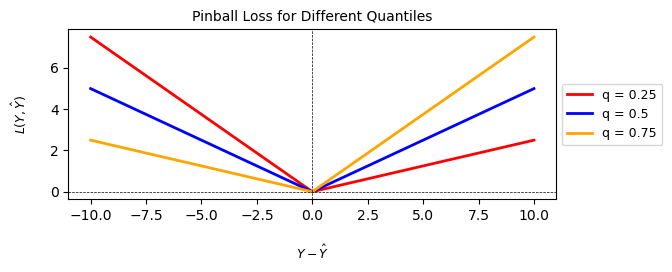
\includegraphics[width=\textwidth]{figures/Pinball_Loss.png}
    % \caption{Caption}
    \label{Pinball_Loss}
\end{figure*}


\textbf{Figure 3.15 Pinball Loss.} Demonstrates the behavior of the Pinball Loss function for three different quantile values $(q = 0.25, 0.5, 0.75)$.
The plot shows how the loss increases linearly with the difference between the predicted value $\hat{Y}$ and the actual value $Y$ for various quantiles, with the loss function being asymmetric around the prediction.

\orangebox{Did you know that...}
{Pinball Loss is also called Quantile Loss and is an L1 Loss when $q=0.5$.}

% ---------- Explained Variance Score ----------
\clearpage
\thispagestyle{regressionstyle}
\section{Explained Variance Score}
\subsection{Explained Variance Score}

The Explained Variance Score is a regression evaluation metric that measures the proportion of variance in the target variable that is captured by the model’s predictions.
It focuses specifically on how well the variability of the data is explained, rather than penalizing systematic biases or a lack of correlation between true and predicted values.

% formula
\begin{center}
    [FORMULA GOES HERE]
\end{center}

Explained Variance Score ranges from -infinity to 1, with 1 indicating that the model explains all variability in the target variable. Negative values suggest the model performs worse
than a horizontal line.

\textbf{Whent to use Explained Variance Score?}

When we need to wnderstanding how well the model explains the variability in the data.

\coloredboxes{
    \item Provides an intuitive measure of how much of the variance in the data is captured by the model.
}
{
    \item Explained Variance Score does not account for systematic offsets between predicted and true values, e.g., the explained variance score between 
    \( y=[1, 2, 3, 4] \) and \( \hat{y}=[8, 9, 10, 11] \). is equal to $1$ despite the predictions being off.
}
